
% 地形の図
\begin{figure}[htbp]
  \begin{tabular}{cc}
    \begin{minipage}[t]{0.42\hsize}
      \begin{center}
      \includegraphics[width=1.0\linewidth,trim={50 50 50 50}, clip]{figure/chapter4/revaluation/flat.png}
      \text{(a) flat terrain}
      \end{center}
    \end{minipage} 
    &
    \begin{minipage}[t]{0.42\hsize}
      \begin{center}
      \includegraphics[width=1.0\linewidth,trim={50 50 50 50}, clip]{figure/chapter4/revaluation/130mm.png}
      \text{(b) up step terrain}
      \end{center}  
    \end{minipage}
    \\
    \begin{minipage}[t]{0.42\hsize}
      \centering
      \includegraphics[width=1.0\linewidth,trim={50 50 50 50}, clip]{figure/chapter4/revaluation/-130mm.png}
      \centering
      \text{(c) down step terrain}
    \end{minipage} 
    &
    \begin{minipage}[t]{0.42\hsize}
      \centering
      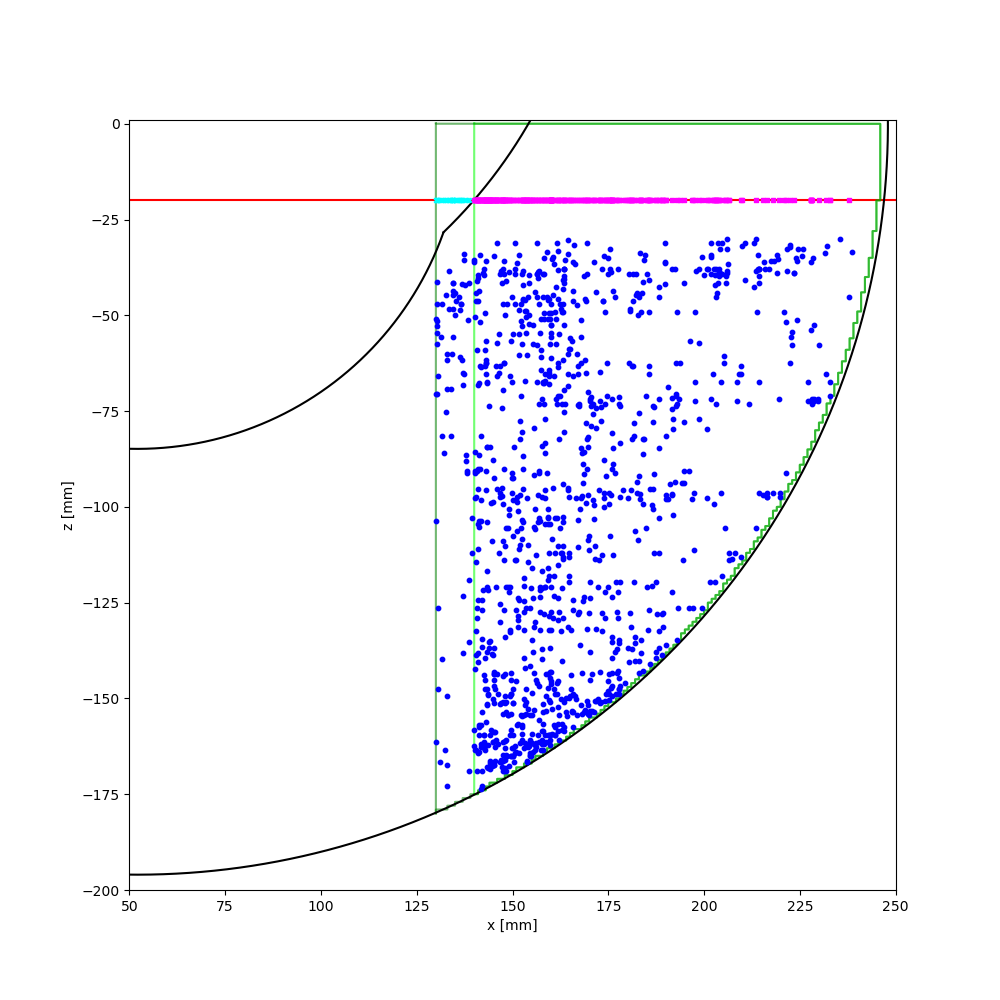
\includegraphics[width=1.0\linewidth,trim={50 50 50 50}, clip]{figure/chapter4/revaluation/15deg.png}
      \centering
      \text{(d) up slope terrain}
    \end{minipage}    
    \\
    \begin{minipage}[t]{0.42\hsize}
      \centering
      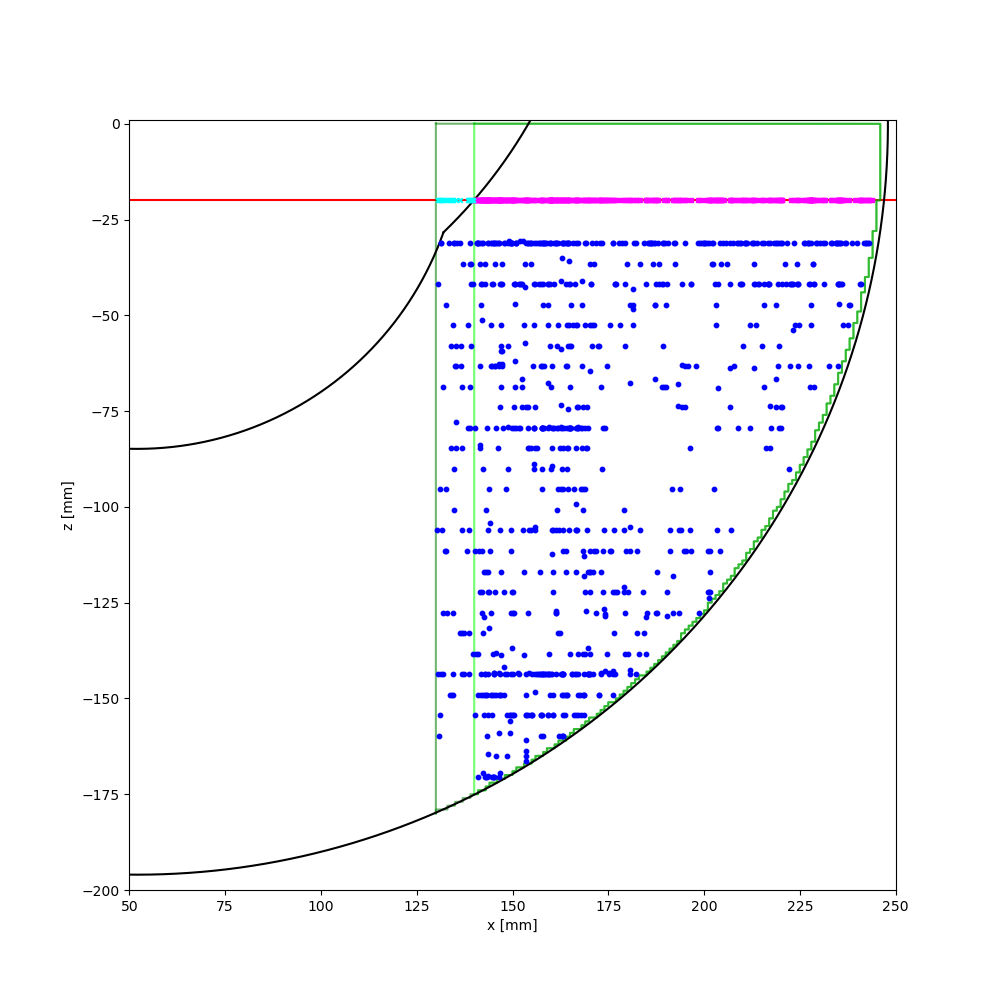
\includegraphics[width=1.0\linewidth,trim={50 50 50 50}, clip]{figure/chapter4/revaluation/-15deg.png}
      \centering
      \text{(e) down slope terrain}
      
    \end{minipage}     
    &
    \\
  \end{tabular}
  \caption{Terrain}
  \label{fig:ch5_simu_terrain} % chktex 24
\end{figure}

\newpage
